\setlength{\parindent}{0pt}
\chapter{\bf APPENDIX} 

\shorthandoff{=}

\begin{figure}[H]
\begin{center}
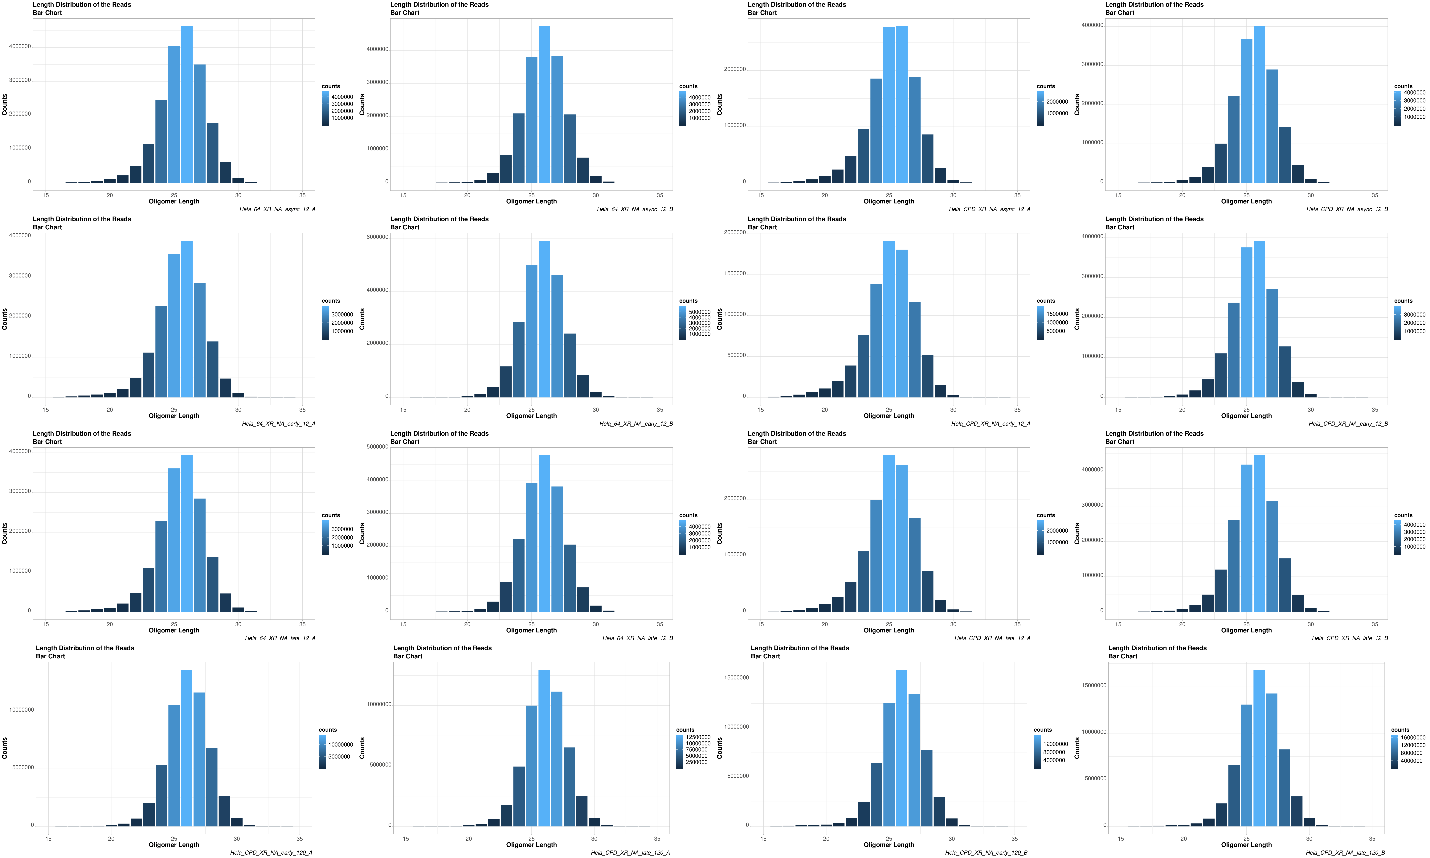
\includegraphics[width=\textwidth]{Chapters/7_appendix/figures/supfig1}
\caption[Length distribution of excised oligomers of XR-seq samples.]{Length distribution of excised oligomers of XR-seq samples after adaptor trimming and duplicate removal. Majority of the oligomers are 26 nucleotides long.}
\label{supfig:length}
\end{center}
\end{figure}


\begin{figure}[H]
\begin{center}
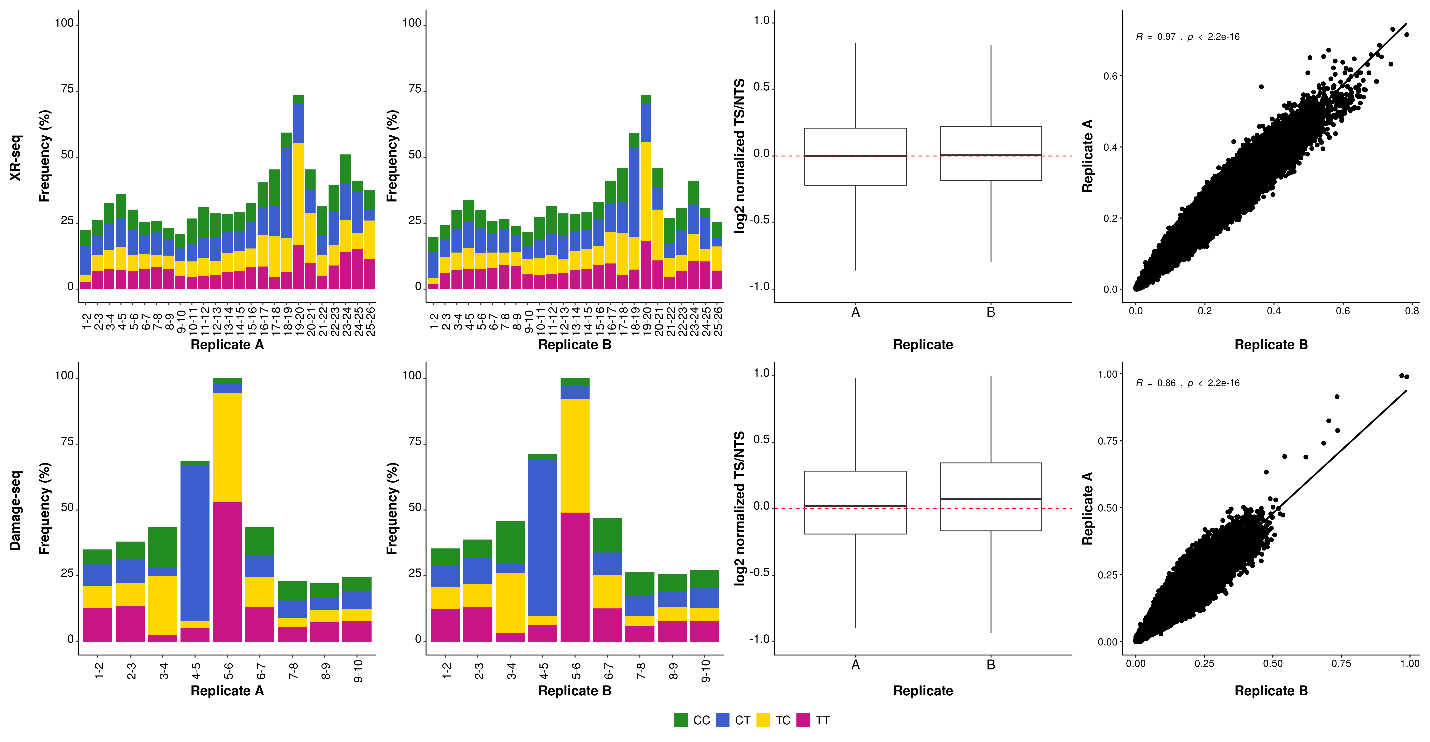
\includegraphics[width=\textwidth]{Chapters/7_appendix/figures/supfig2}
\caption[Control figures of (6-4)PP asynchronized samples at 12 minutes.]{Control figures of (6-4)PP asynchronized samples at 12 minutes. Column 1 is the correlation plot of the biological replicates (A \& B). Column 1 and 2 displays the dinucleotide composition frequency of replicate A and B, respectively. Column 3 is the log2 transformed TS/NTS ratios of replicate A and B. Row 1 is the results of XR-seq samples, and row 2 is the results of Damage-seq samples. Column 4 is the correlation plot of the biological replicates (A \& B). Correlation coefficient is calculated by Spearman’s rank correlation test.}
\label{supfig:control1}
\end{center}
\end{figure}


\begin{figure}[H]
\begin{center}
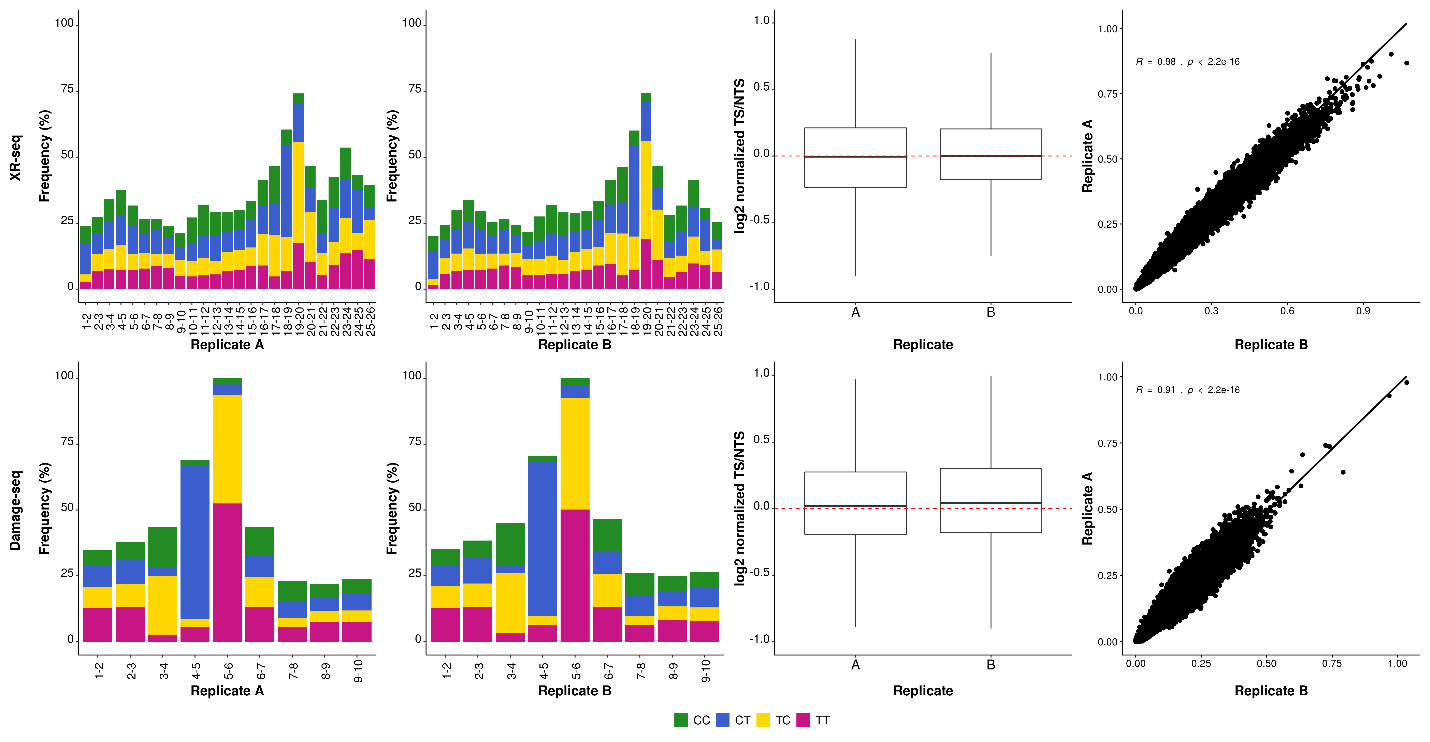
\includegraphics[width=\textwidth]{Chapters/7_appendix/figures/supfig3}
\caption[Control figures of (6-4)PP early phased samples at 12 minutes.]{Control figures of (6-4)PP early phased samples at 12 minutes. Column 1 is the correlation plot of the biological replicates (A \& B). Column 1 and 2 displays the dinucleotide composition frequency of replicate A and B, respectively. Column 3 is the log2 transformed TS/NTS ratios of replicate A and B. Row 1 is the results of XR-seq samples, and row 2 is the results of Damage-seq samples. Column 4 is the correlation plot of the biological replicates (A \& B). Correlation coefficient is calculated by Spearman’s rank correlation test.}
\label{supfig:control2}
\end{center}
\end{figure}


\begin{figure}[H]
\begin{center}
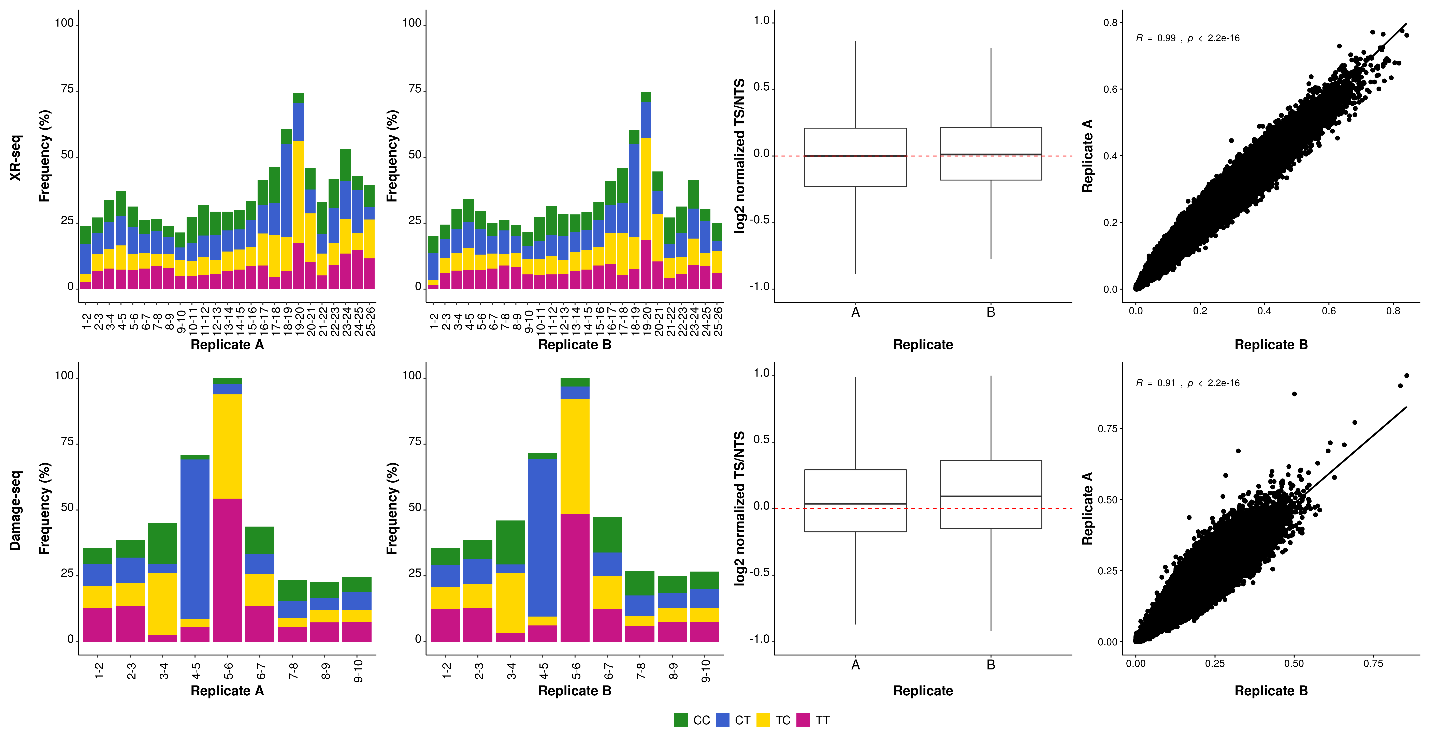
\includegraphics[width=\textwidth]{Chapters/7_appendix/figures/supfig4}
\caption[Control figures of (6-4)PP late phased samples at 12 minutes.]{Column 1 is the correlation plot of the biological replicates (A \& B). Column 1 and 2 displays the dinucleotide composition frequency of replicate A and B, respectively. Column 3 is the log2 transformed TS/NTS ratios of replicate A and B. Row 1 is the results of XR-seq samples, and row 2 is the results of Damage-seq samples. Column 4 is the correlation plot of the biological replicates (A \& B). Correlation coefficient is calculated by Spearman’s rank correlation test.}
\label{supfig:control3}
\end{center}
\end{figure}


\begin{figure}[H]
\begin{center}
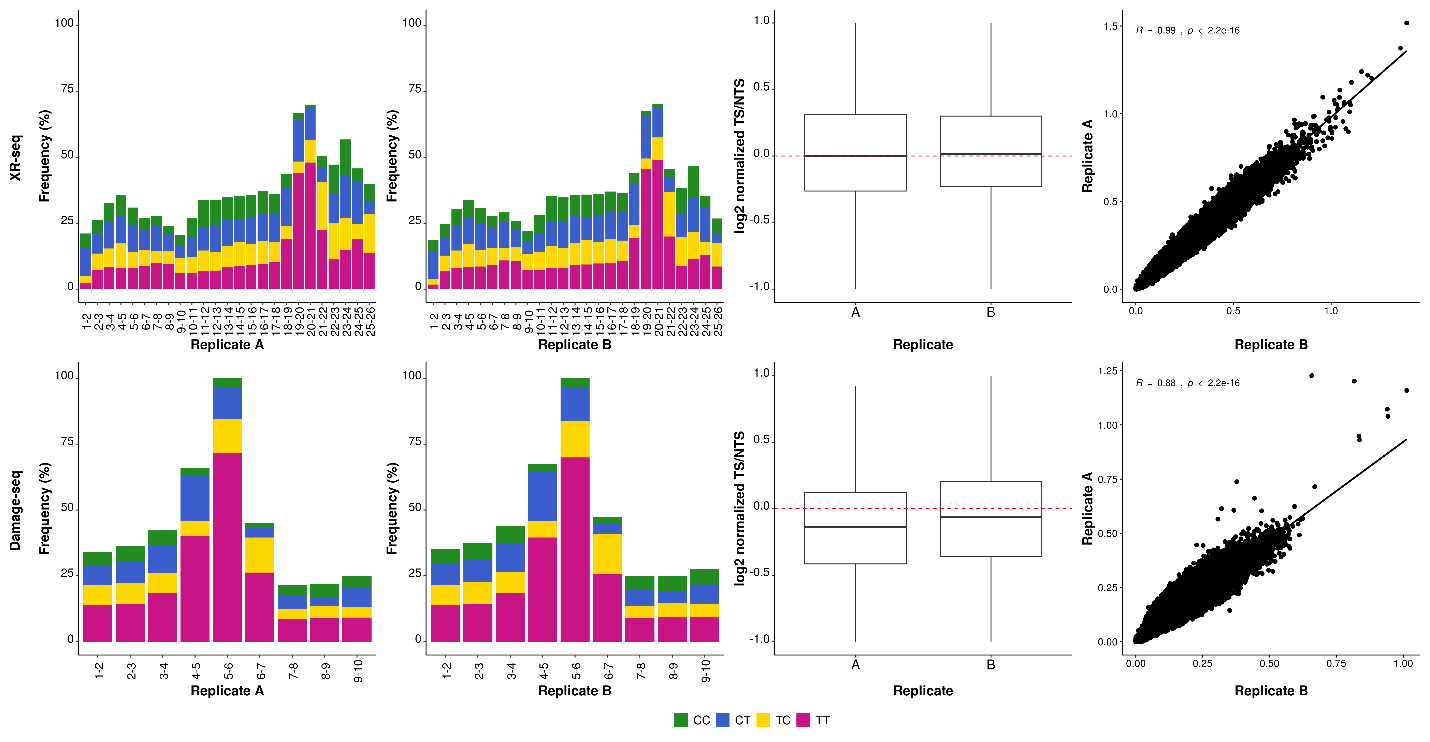
\includegraphics[width=\textwidth]{Chapters/7_appendix/figures/supfig5}
\caption[Control figures of CPD asynchronized samples at 12 minutes.]{Control figures of CPD asynchronized samples at 12 minutes. Column 1 is the correlation plot of the biological replicates (A \& B). Column 1 and 2 displays the dinucleotide composition frequency of replicate A and B, respectively. Column 3 is the log2 transformed TS/NTS ratios of replicate A and B. Row 1 is the results of XR-seq samples, and row 2 is the results of Damage-seq samples. Column 4 is the correlation plot of the biological replicates (A \& B). Correlation coefficient is calculated by Spearman’s rank correlation test.}
\label{supfig:control4}
\end{center}
\end{figure}


\begin{figure}[H]
\begin{center}
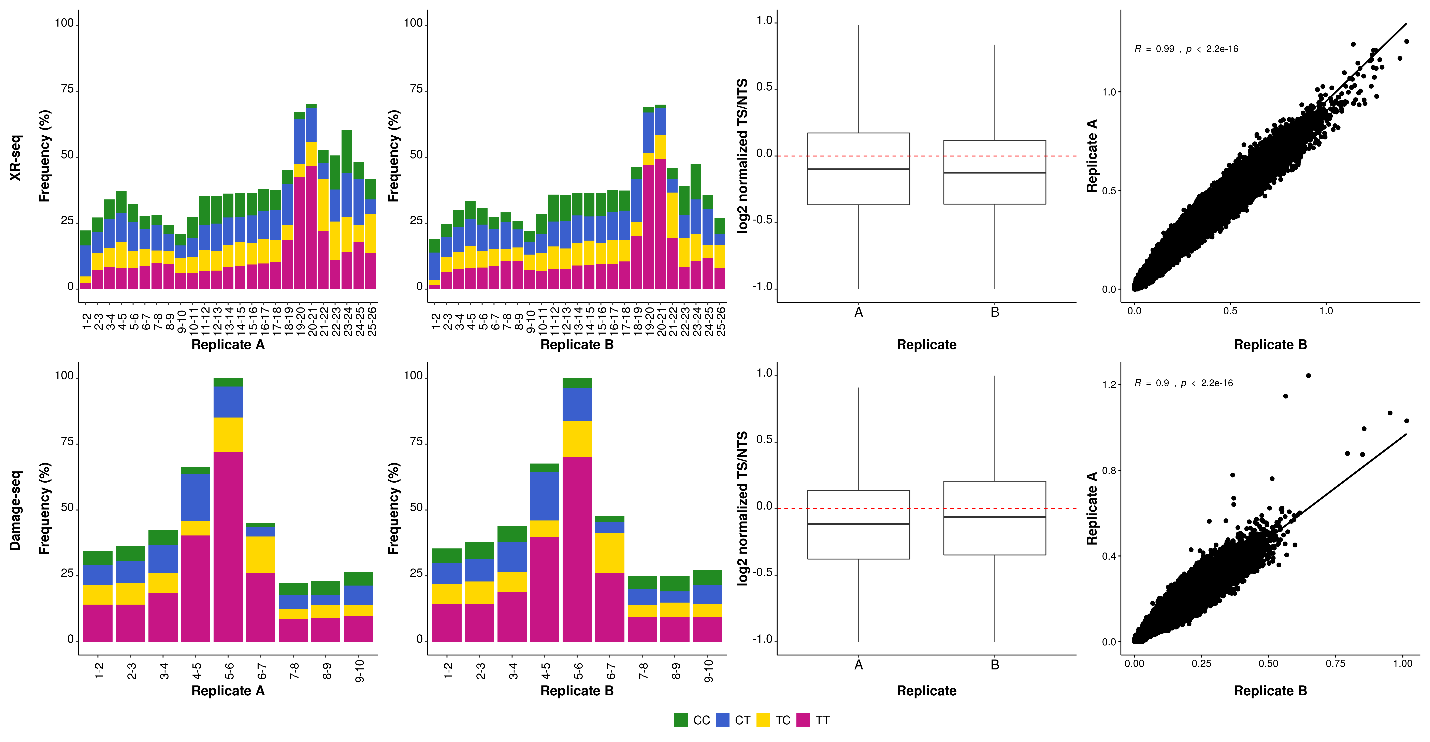
\includegraphics[width=\textwidth]{Chapters/7_appendix/figures/supfig6}
\caption[Control figures of CPD early phased samples at 12 minutes.]{Control figures of CPD early phased samples at 12 minutes. Column 1 is the correlation plot of the biological replicates (A \& B). Column 1 and 2 displays the dinucleotide composition frequency of replicate A and B, respectively. Column 3 is the log2 transformed TS/NTS ratios of replicate A and B. Row 1 is the results of XR-seq samples, and row 2 is the results of Damage-seq samples. Column 4 is the correlation plot of the biological replicates (A \& B). Correlation coefficient is calculated by Spearman’s rank correlation test.}
\label{supfig:control5}
\end{center}
\end{figure}


\begin{figure}[H]
    \begin{center}
    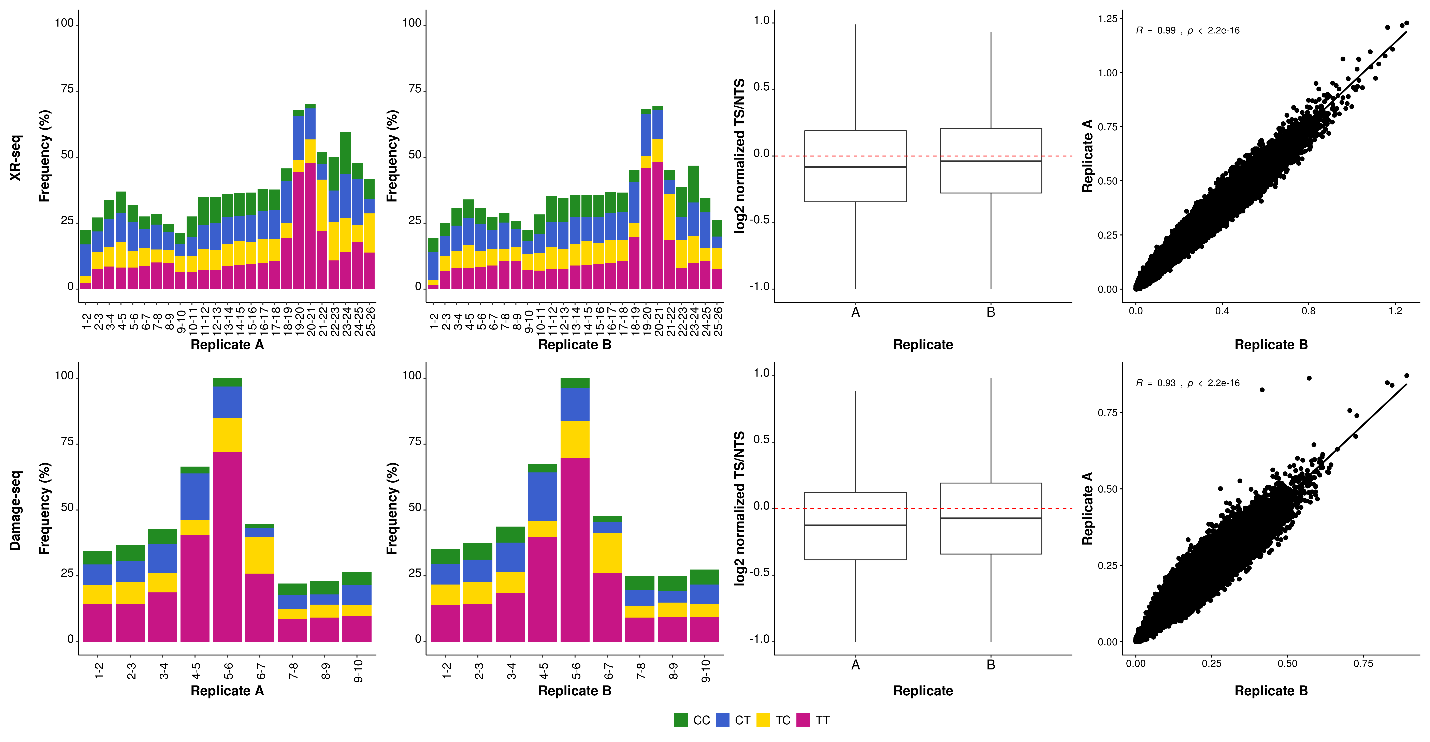
\includegraphics[width=\textwidth]{Chapters/7_appendix/figures/supfig7}
    \caption[Control figures of CPD late phased samples at 12 minutes.]{Control figures of CPD late phased samples at 12 minutes. Column 1 is the correlation plot of the biological replicates (A \& B). Column 1 and 2 displays the dinucleotide composition frequency of replicate A and B, respectively. Column 3 is the log2 transformed TS/NTS ratios of replicate A and B. Row 1 is the results of XR-seq samples, and row 2 is the results of Damage-seq samples. Column 4 is the correlation plot of the biological replicates (A \& B). Correlation coefficient is calculated by Spearman’s rank correlation test.}
    \label{supfig:control6}
    \end{center}
    \end{figure}

\begin{figure}[H]
    \begin{center}
    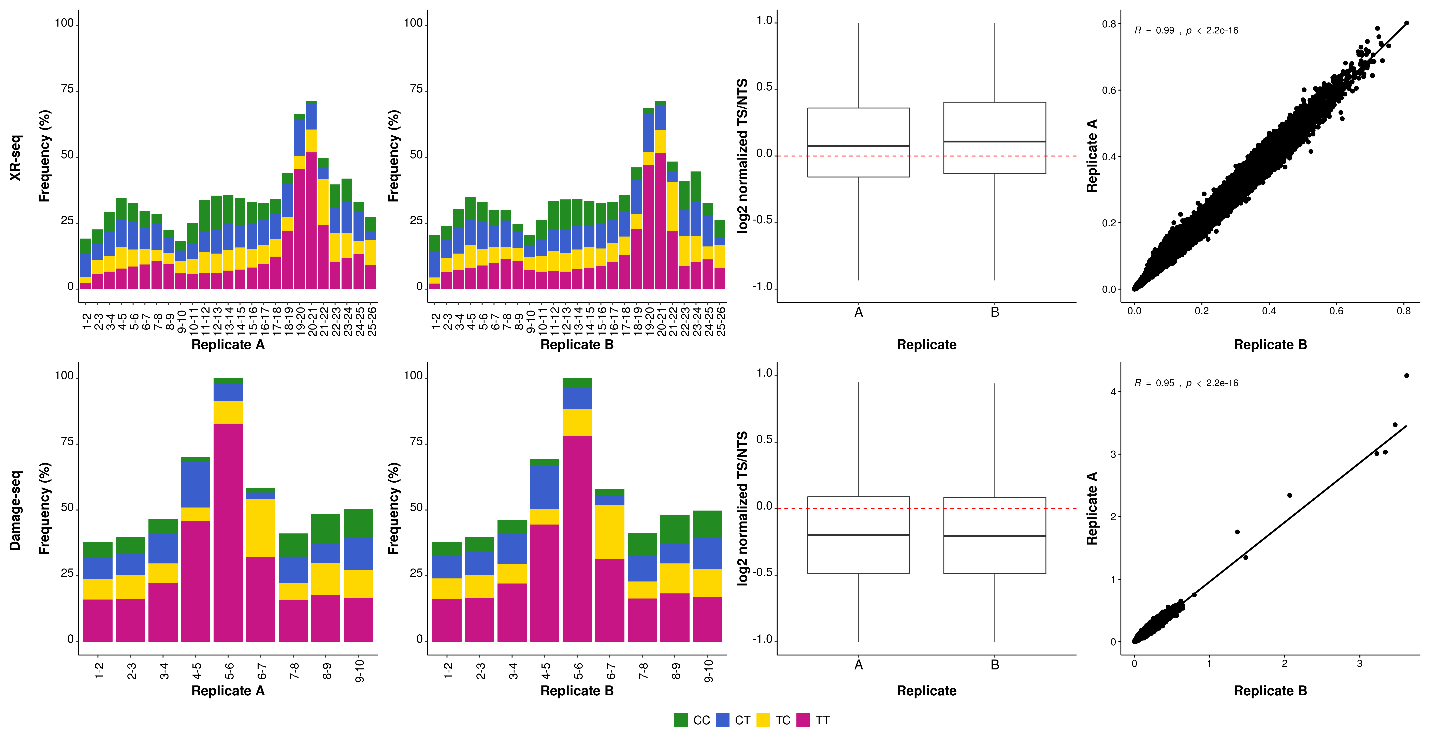
\includegraphics[width=\textwidth]{Chapters/7_appendix/figures/supfig8}
    \caption[Control figures of CPD early phased samples at 120 minutes.]{Control figures of CPD early phased samples at 120 minutes. Column 1 is the correlation plot of the biological replicates (A \& B). Column 1 and 2 displays the dinucleotide composition frequency of replicate A and B, respectively. Column 3 is the log2 transformed TS/NTS ratios of replicate A and B. Row 1 is the results of XR-seq samples, and row 2 is the results of Damage-seq samples. Column 4 is the correlation plot of the biological replicates (A \& B). Correlation coefficient is calculated by Spearman’s rank correlation test.}
    \label{supfig:control7}
    \end{center}
    \end{figure}

\begin{figure}[H]
    \begin{center}
    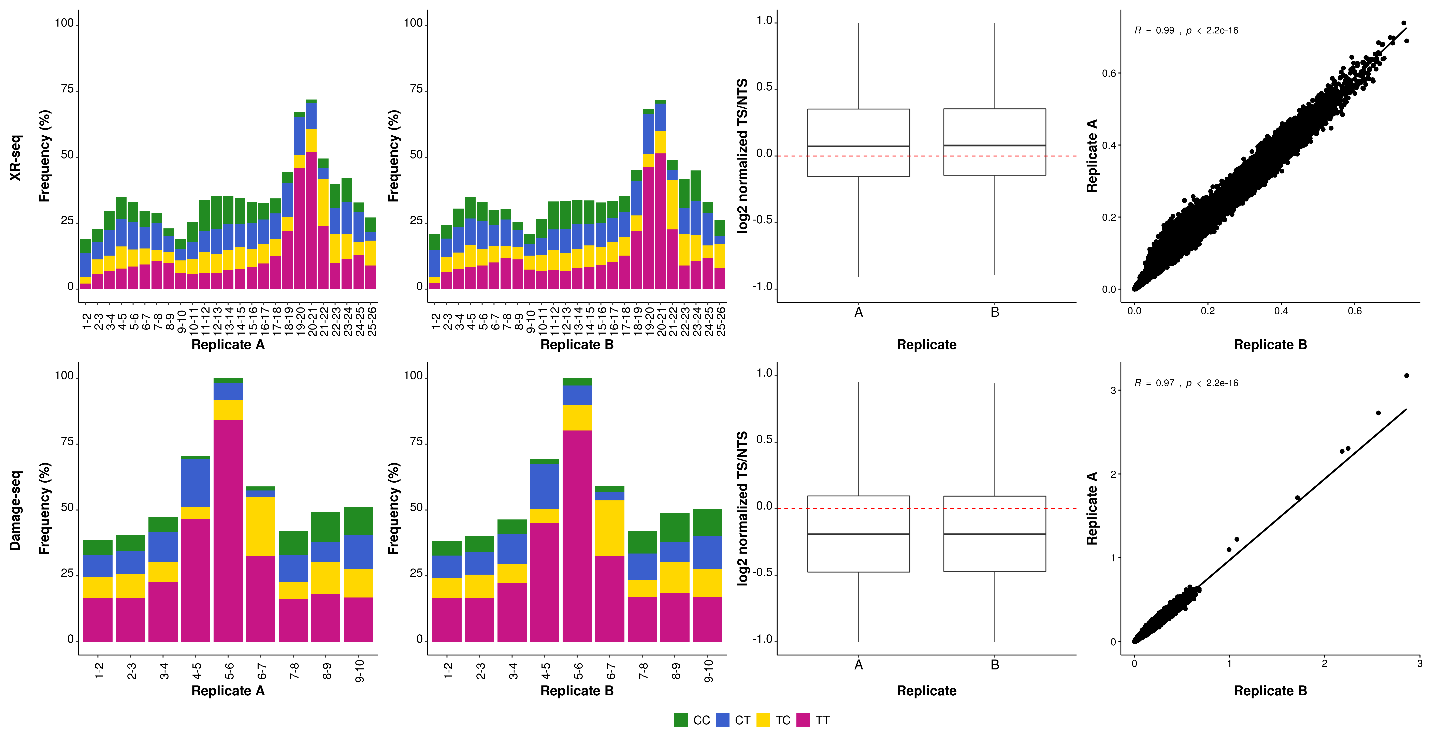
\includegraphics[width=\textwidth]{Chapters/7_appendix/figures/supfig9}
    \caption[Control figures of CPD late phased samples at 120 minutes.]{Control figures of CPD late phased samples at 120 minutes. Column 1 is the correlation plot of the biological replicates (A \& B). Column 1 and 2 displays the dinucleotide composition frequency of replicate A and B, respectively. Column 3 is the log2 transformed TS/NTS ratios of replicate A and B. Row 1 is the results of XR-seq samples, and row 2 is the results of Damage-seq samples. Column 4 is the correlation plot of the biological replicates (A \& B). Correlation coefficient is calculated by Spearman’s rank correlation test.}
    \label{supfig:control8}
    \end{center}
    \end{figure}


                                                        

